\documentclass[a4paper,twoside]{article}

\usepackage{epsfig}
\usepackage{subcaption}
\usepackage{calc}
\usepackage{amssymb}
\usepackage{amstext}
\usepackage{amsmath}
\usepackage{amsthm}
\usepackage{multicol}
\usepackage{pslatex}
\usepackage{apalike}
\usepackage[bottom]{footmisc}
\usepackage[table,xcdraw]{xcolor}
\usepackage{SCITEPRESS}     % Please add other packages that you may need BEFORE the SCITEPRESS.sty package.
\usepackage{graphics}
\usepackage{lscape}
\usepackage{float}
\usepackage{url}
\usepackage{multirow}
\begin{document}
\title{An Open Tool-set for Simulation, Design-space Exploration and Optimization of Supply Chains and Inventory Problems}

%\title{Case Study-based Evaluation of the Suitability and Efficacy of Different Open-source Metamodeling approaches and Optimizers for Simulation-based Digital Twins}

%\author{\authorname{Tushar Lone\orcidAuthor{0000-0003-0008-0429}, Lekshmi P.\orcidAuthor{0000-0001-5464-6032},  and Neha Karanjkar\orcidAuthor{0000-0003-3111-1435}}
%\affiliation{Indian Institute of Technology Goa, India}
%\email{\{lekshmi20231101, tushar20231102, nehak\}@iitgoa.ac.in}
%}

\keywords{Supply Chains, Inventory, Discrete-Event Simulation, Python, Meta-models, Optimization}

\abstract{Simulation plays a key role in the design, analysis and optimization of supply chain systems.  While analytical models may suffice for very simple systems with ideal behavior, a detailed stochastic discrete-event model becomes necessary to capture component behaviors and complex structures of modern supply chains with reasonable accuracy.  However,  simulation-based optimization is often difficult owing to the large number of decision variables, the computational cost of performance estimation using multiple stochastic simulation runs and non-convex, black-box objective functions.  Meta-models can assist in the optimization process, but the process of choosing the right meta-model type, the number of data points to build the meta-model and the right optimizer can be non-trivial and can significantly affect the results.  
%
This paper presents the design overview of  \textbf{InventOpt} - a Python-based, open tool-set for simulation, design space exploration and optimization of supply chains and inventory systems. InventOpt consists of a Python library of component models  that can be instantiated and connected together to model and simulate complex supply chains. In addition, InventOpt contains a GUI-based tool to assist the user in planning design of experiments, visualizing the objective functions over a multi-dimensional design space, building meta-models by selecting an appropriate number of data points and performing an optimization over these meta-models to identify promising regions and optimal points in the design space. In order to validate the proposed approach, we present a detailed case study of simulation-based optimization of inventory levels in a supply chain with 8 design parameters. We present our observations regarding  choices such as the type of meta-model, number of simulation runs used for building the meta-model, the choice of optimizer and the trade-off between computational cost and quality of results. Each step in this case study has been implemented using open Python libraries. The case study serves as a basis for the design and implementation of InventOpt.}

\onecolumn \maketitle \normalsize \setcounter{footnote}{0} \vfill

%%%%%%%%%% %%%%%%%%%% %%%%%%%%%% %%%%%%%%%% %%%%%%%%%% %%%%%%%%%% %%%%%%%%%% %%%%%%%%%% %%%%%%%%%% %%%%%%%%%% %%%%%%%%%% %%%%%%%%%% %%%%%%%%%% %%%%%%%%%%
\section{\uppercase{Introduction}}
\label{sec:introduction}
A supply chain (SC) is a network of entities (such as manufacturers, distributors, transporters, warehouses etc) involved in producing, transporting, storing and distributing goods and services. The primary goals in the design of a supply chain are to minimize risk, maximise net profits and satisfy end-user demands. \cite{chopra2007supply}. Modern supply chains have complex structures, often spanning multiple continents and a large set of interconnected entities with diverse behaviors. While deterministic analytical models suffice to analyze simple supply chains, the use of detailed simulation models becomes imperative to capture complex behaviors and dependencies between its components with reasonable accuracy. Simulation allows managers to mitigate risks by evaluating what-if scenarios and provides a mechanism to identify bottlenecks and optimize processes for better profits. Most importantly, simulation-based analysis can provide insights into how different factors, such as lead times, demand variability and inventory levels can impact performance and net profit.
System Dynamics (SD), Discrete-event Simulation (DES), Monte-Carlo Simulation and Hybrid simulation are some approaches used for modeling and studying supply chains. \cite{Mustafee}. 
%
While there exist several commercial tools (such as AnyLogic, FLEXSIM, Arena, IBM Supply Chain solutions), there is a dearth of open libraries in popular programming languages for supply chain design and optimization.  General-purpose discrete-event simulation frameworks (such as Python's SimPy library \cite{SimPy} ) can be used for building simulation models of supply chains. However, validation constitutes a significant fraction of model development time. Having an open library of  pre-built, validated parameterized component models can be very useful in rapid modeling and design space exploration.  

In a similar vein, while there exist open, general-purpose libraries for optimization, simulation-based optimization of supply chains is a non-trivial task because of the enormity of the design space and the computational expense of multiple simulation runs. 
%
To illustrate with an example, suppose a system has 10 design variables whose values we wish to find within a some given range for maximising a performance metric (say average net profit).  Some of these design variables might be integer/discrete valued and others may be continuous. If we assume each variable can take one out of  just 10 possible values/levels, the design space will still have $10^{10}$ (10 Billion) points  that we need to explore. Since the simulation model is stochastic, long-run average performance estimates (such as the average monthly profit) at a single design point can be obtained by averaging the results over multiple simulation runs with distinct randomization seeds. If each simulation run is assumed to take a millisecond, the time required for exhaustively evaluating the entire design space will still be prohibitive. Although there exists no analytical expression for the objective function or its derivatives in such problems (black-box optimization), the objective functions often display low-order trends and can be mimicked by multi-dimensional polynomial surfaces. Meta-model based optimization approaches exploits this aspect.

A \textbf{Meta-model} is a function that approximates the detailed simulation model and is computationally less expensive to evaluate \cite{barton2020tutorial}. If $X = (x_1, x_2, \dots, x_n)$ represents a point in the n-dimensional design space, and multiple runs of the the stochastic simulation model estimate some average performance metric $f(X)$, then the meta-model $g(X)$ is an (ideally smooth) function which approximates $f$.  It can be constructed by measuring $f$ at only a few  points in the design space and performing some form of interpolation or regression between them. As the number of measurement points increases, the meta-model typically becomes more and more accurate unless it suffers from over-fitting (leading to drastic overshoots or oscillations in the meta-model surface in-between measured points). The meta-model should ideally be smooth and significantly easier/faster  to evaluate than the detailed simulation-based measurement.  Continuous gradient-based optimizers can then be applied over the meta-model surface $g$ to quickly identify promising areas in the design space for further exploration.  Response Surface Models (RSM), Radial Basis Functions, Kriging (Gaussian Process Regression), and Neural Networks (NN) are some meta-models types that are used in various application domains.  Neural Networks and Kriging are popular and considered to have better accuracy \cite{barkanyi2021modelling}.  \textbf{Kriging}, also known as \textbf{Gaussian Process Regression }(GPR) is a spatial correlation meta-model \cite{kleijnen2009kriging,ankenman2008stochastic}. It uses a \textit{kernel function} to represent the  correlation between different input parameter values. Euclidean distance, Gaussian kernel, Radial Basis Function (RBF), and periodic RBF are some examples of kernel functions used in Kriging. A \textbf{Neural Network} meta-model is built using a neural network architecture (for example, a multi-layer feed-forward network) with the measured points as training data to learn and mimic the input-output relation. It is then used to approximate the performance measures of the system at a given point. The process of selecting the meta-model type, tuning it and selecting the right optimizer for optimizing over for it are nuanced and problem-dependent choices. 

This paper presents an overview of \textbf{InventOpt} - a Python-based open library and tool-set we propose to build for supply chain and inventory systems simulation and meta-model based optimization. InventOpt primarily consists of  a library of component models for simulating supply chains. These component models are built using Python's SimPy library, and can be instantiated, configured and connected together to model complex supply chains. In addition, InventOpt will include a GUI-based tool for guided design-space exploration, meta-model tuning and optimization. To make suitable design choices for InventOpt (such as the meta-model type, number of measurement points relative to the size of the design space, and the choice of the optimization algorithm) that are specifically suited for simulation-based optimization of supply chains, we perform a detailed case study.  In this case study we consider the problem of optimizing the net average profit in a particular supply chain with a large number of design parameters that control the inventory thresholds and reorder points at various nodes.  We build a modular simulation model and perform computational cost versus accuracy trade-off analysis to determine the number of simulation runs suitable for evaluating each point in the design space.  We then perform detailed simulation-based evaluation at points in the 8-dimensional design space along a regular grid pattern to identify the optimum points/regions with respect to a single objective function. This data serves as a reference for evaluating the meta-model based approach. We separate the measured points into a training set and a test set. Training sets containing various fractions of the total measured points are used to build two kinds of meta-models: NN and GPR. We then perform meta-model based optimization using multiple local optimization algorithms with random restarts and present our observations and insights regarding the impact of these design choices on the quality of the results and the computational effort. We use open Python libraries at each step of the process (namely, SimPy \cite{SimPy} for discrete-event simulation, SciPy.Optimize \cite{2020SciPy-NMeth} for optimization, and the Scikit library for building the meta-models). This case study serves as a basis for generalization into a tool-set for supply chain simulation and optimization. 

The rest of the paper is organized as follows: in Section \ref{sec:relatedwork}, we present a summary of related work and existing tools for supply chain simulation and optimization. We then present an overview of InventOpt and discuss its proposed features and implementation plan in Section \ref{sec:proposedtool}.  Section \ref{sec:casestudy} presents the detailed case study and Section \ref{sec:results} summarizes the observations and insights gained from the case study towards the implementation of InventOpt.

%The supply chain optimization is done by building its analytical or simulation model in computer memory and optimizing over different supply chain parameter values (design space). The analytical model helps examine the standard behaviour of the supply chains. The simulation model captures the supply chain's complex, stochastic nature and dynamic behaviour. It can be built using Discrete Event Simulation (DES) libraries like SimPy \cite{SimPy}. SimPy is an open-source Python library to model any systems in computer memory, is generalized to construct a discrete event simulation model of a system and is not specifically targeted to build supply chain networks. 
%OpenBoxes, Zoho, OpenLMIS, and Sonatype, are a few of the many online tools and platforms available for the supply chain management. These have free and paid features and services. Their products and software tools focus more on managing the supply chain than optimizing it. Section \ref{sec:relatedwork} presents a comprehensive overview of platforms and tools that offer services for modeling and analyzing supply chains. 
%anyLogistix (anyLogic), Simio, and Supply Chain Guru are commercial tools to simulate supply chains that provide various analysis tools, such as optimization and statistical analysis. Still, these are paid tools and cannot be accessed for free. \textit{supplychainpy} is an open-source Python library for simulating and analyzing supply chain systems and inventories with Monte Carlo simulation. However, users need Python programming knowledge to invoke and implement a simulation model for the supply chain and analyze it. We propose to build a framework consisting open-source Python library built on top of SimPy and a GUI-based tool that aids the user in the complete process of supply chain creation to optimization. A user can directly import and instantiate the proposed library to model various supply chain networks with different behaviours and parameters. 
%After building a simulation model for a supply chain network, validation and performance analysis of the model in terms of time complexity and correctness are crucial since the simulation model often inherits the supply chain complexity.
%The validation and performance analysis of a simulation model for a supply chain network is crucial, given that the model typically inherits the complexity of the supply chain. This is particularly true in terms of time complexity and correctness. Due to the potentially vast design space and the need for multiple simulation runs to estimate expected performance measures in a stochastic model, the optimization task is computationally demanding. For example, with ten design variables and just two choices for each parameter value, $2^{10} = 1024$ different design points exist. So the design space is vast, and each simulation run can be computationally costly.
%Furthermore, the optimizers call upon objective functions that require running the simulation model for different parameter values. The optimizer invokes the objective function with continuous parameter values, and the simulation model often has mixed discrete and continuous parameter values. Therefore, most continuous optimizers do not work well for simulation model optimization.
%Moreover, the gradient information is not readily available when optimizing a simulation model. One solution is to use Meta-models. These models are typically used to approximate the relationships between inputs parameters and outputs (performance measures) of the simulation model in a computationally efficient manner. There exists a correlation between the input parameters and output performance measures of the simulation model, and they display discernible patterns. Therefore a Meta-model can exploit its gradient information for the optimizers to work well. We introduce the meta-models utilized in the case-study.
%Meta-models are built on top of the simulation model, and they are less accurate and more time efficient than the simulation model. It is built by sampling a few points from the simulation model design space called training points. It then approximates a continuous surface to training points by exploiting the input-output relationship. The Meta-model $g$ is then used to estimate the performance measure for any input parameter values in the design space instead of the computationally expensive simulation model $f$. 

%This study aims to develop a framework comprising libraries and graphical user interface (GUI) tools that enable the user to model a supply chain network with a visual interface in performing meta-model-based optimization. Several critical tasks must be performed during the meta-model-based optimization process, including selecting an appropriate meta-model, determining the required number of training points, selecting an appropriate sampling method, estimating the necessary number of simulations, and determining the optimal duration of the simulation. Often, these design decisions are not straightforward to follow during the Meta-model based supply chain optimization. The proposed tools will aid the user at each step of these decisions.

%This paper presents a case study that illustrates the individual components and steps of the proposed framework that can aid in making significant decisions about meta-model-based optimization. The case study comprises an inventory optimization problem in the supply chain network. It is modeled, simulated and optimized using the meta-model-based approach, and obtained results and insights are presented. The rest of the paper is organized as follows: in section \ref{sec:relatedwork}, we discuss related work to ours. The proposed framework and GUI-based tool InventOpt is introduced in section \ref{sec:proposedtool}. The section \ref{sec:casestudy} discusses the case study and illustrates the flow of the components in the proposed tool. Finally, section \ref{sec:results} discusses the results and insights obtained from the experiment and concludes the paper.




%%%%%%%%%% %%%%%%%%%% %%%%%%%%%% %%%%%%%%%% %%%%%%%%%% %%%%%%%%%% %%%%%%%%%% %%%%%%%%%% %%%%%%%%%% %%%%%%%%%% %%%%%%%%%% %%%%%%%%%% %%%%%%%%%% %%%%%%%%%%
\section{\uppercase{Related Work}}
\label{sec:relatedwork}
This section presents an overview of the commercial and free/open tools available for various aspects of supply chain design and analysis. Commercial tools such as Anylogic \cite{Anylogic} (and its logistics-specific solution, Anylogicstix),  FLEXSIM \cite{Flexsim}, and Arena \cite{Arena} support supply chain simulation. Anylogic supports the development of models using three approaches: DES, agent-based and system dynamics. AnyLogic and FlexSim also support optimization, which is built on top of the OptQuest \cite{OptQuest} optimization engine.  IBM supply chain solutions \cite{IBM} is a suite that provides AI-powered solutions for supply chain optimization. 
%
Among open-source libraries for supply chain simulation, MiniSCOT  \cite{miniSCOT} is a Python package for simulating supply chain models that was developed by Amazon and released as open-source in 2021 under an Apache licence. However it does not contain any documentation or usage guidelines and the latest commit was in 2021. \texttt{supplychainpy} \cite{Supplychainpy} is another Python library for simulating and analyzing supply chains which is primarily meant to replace existing spreadsheet-based workflows. It accepts demand data from a csv file and can generate performance metrics based on analytical formulae. It also supports a basic Monte Carlo simulation that generates normally distributed demand, based on the historical data in the csv file. The demand for each item/unit is then used to model a probable transaction history. Only single/independent inventory nodes can be modeled, without considering their dependencies or complex interconnections. For this a simple Monte-Carlo simulation is sufficient and a detailed discrete-event simulation is not required. The proposed library of InventOpt differs from this as it would provide detailed component models that can be connected together and simulated as concurrent entities using a discrete-event simulation approach.
%
For design exploration and gaining insights from the multi-dimensional simulation data, visualization is an important step. InventOpt will provide a GUI interface to visualise 3D slices of multi-dimensional data. For a similar purpose, Hypertools \cite{Hypertools} is an existing Python library for visualizing high-dimensional data. It also supports dimensionality reduction using the Principal Component Analysis (PCA) technique. 

 
%%%%%%%%%% %%%%%%%%%% %%%%%%%%%% %%%%%%%%%% %%%%%%%%%% %%%%%%%%%% %%%%%%%%%% %%%%%%%%%% %%%%%%%%%% %%%%%%%%%% %%%%%%%%%% %%%%%%%%%% %%%%%%%%%% %%%%%%%%%%
\section{\uppercase{Overview of} InventOpt}
\label{sec:proposedtool}
InventOpt is a Python-based, open tool-set targeted for simulation, design exploration and optimization of supply chain and inventory problems. This section describes the features and components that are currently implemented (illustrated by the case study in Section \ref{sec:casestudy}) as well as those planned to be implemented in future. InventOpt consists of the following key components:

%\begin{itemize}[leftmargin=*]
 %   \item 
    \vspace{0.2em}
    \noindent $\bullet$ \textbf{Component Library:} An open Python library of parameterized component models to model the behavior of individual components in supply chains such as inventory nodes, distributors, manufacturers and demand/customer arrivals. These components can be instantiated and connected together  to model supply chains with complex structures. In addition, a user will be able to derive classes from the in-built component classes to describe non-standard or custom behaviors in a modular and extensible way. Simulation of the instantiated components is performed using Python's SimPy DES library.
       %\item 
     
     \vspace{0.2em}\noindent $\bullet$ \textbf{Routines for Accuracy-Cost Trade-off:} Once a simulation model has been built, it is necessary to understand the trade-off between model accuracy and computational cost. Since the model is stochastic, it is necessary to perform multiple simulation runs to obtain performance estimates. InventOpt provides routines for automatically generating the computational cost versus accuracy trade-off plots at specified points in the design space so that a user can predict and budget the computing time for efficient design space exploration. This is illustrated in our case study presented in Section \ref{sec:casestudy}.
    
    %\item 
     \vspace{0.2em}\noindent $\bullet$ \textbf{Tool-set for Design Space Exploration}: InventOpt will provide a GUI interface that would allow a user to describe the bounds on design variables, scripts to sample the multi-dimensional design space by performing parallel simulations efficiently at multiple points and visualize the data over a multi-dimensional space. This step is critical for gaining insight on the effect of various design variables on performance measures. It also assists in model validation by allowing the user to visually check for expected trends and unexpected outliers, possibly pointing to bugs in the model. In the current implementation (discussed in Section \ref{sec:casestudy}) this functionality is provided via Python routines and scripts, and a GUI interface will be added in future. 
     
    %\item 
     \vspace{0.2em}\noindent $\bullet$ \textbf{Meta-model generation routines}: InventOpt provides a basic GUI interface to build and visualize meta-models for optimization. In future implementation a GUI will support the user in selecting the meta-model type, and tuning it by specifying the number of data points to build the meta-model and the split between training and test data points for measuring the extent of fit between the original data and the meta-model. The tool will also provide recommendations or default values for these choices. Once a meta-model is built, goodness of fit measures (such as sum-of-squared errors) are reported.  
    %
     The GUI interface also allows the user to visualize the measured points superimposed on the meta-model. Since the meta-model is a multidimensional surface, one possible way is to visualize it as 3D slices with two axes specified at a time and the other axes values being fixed via user input from interactive sliders. Figure \ref{fig:DataVis_slice} shows a screenshot of such a visualization interface we have implemented for this purpose. Using this interface, the user can select two dimensions at a time to visualize a 3D slice of the meta-model superimposed on the measured simulation data. For the other dimensions, the user can select a range of values or a particular value using interactive sliders.
               
    %\item
     \vspace{0.2em}\noindent $\bullet$ \textbf{Guided Optimization}: Once a meta-model has been built, continuous optimizers can be applied to rapidly identify promising regions for further exploration or to directly perform an optimization over the meta-model. InventOpt will provide the user an option to select and use one of several optimization algorithms. 
     %For this, libraries such as \texttt{scipy.optimize} and other parallel black-box optimization libraries can be utilized in the back-end.
     For this, libraries such as \texttt{scipy.optimize} and parallel optimization packages such as \textit{Pymoo} \cite{pymoo} and \textit{ParMoo} \cite{chang_2022} can be utilized in the back-end. 
     While the case study presented in Section \ref{sec:casestudy} shows the use of local optimizers only, future implementations will provide the option of using global optimizers (such as Simulated Annealing) also. Through a simple GUI interface, InventOpt will suggest optimizers and random restart points to the user based on heuristics and the measured simulation data. It will generate convergence plots for multiple runs of the optimizers and provide various statistics for assisting in the optimization process. This process can be performed iteratively: optimizers can be used to identify good regions in the design space, which can be narrowed down for fine-grained exploration to build meta-models and optimize in these sub-regions. 
     % \end{itemize}
      
    To establish and validate the suitability of the meta-model based approach, we perform a detailed case study described in the next section. The problem addressed in the case study is representative of a broad class of problems in supply chain optimization and the insights gained can be translated into a general approach incorporated into the InventOpt tool.
    %This case study serves as a basis for the design of InventOpt. While the optimum approach may be specific for each problem instance, we expect that 
    
    
  
 

%%%%%%%%%% %%%%%%%%%% %%%%%%%%%% %%%%%%%%%% %%%%%%%%%% %%%%%%%%%% %%%%%%%%%% %%%%%%%%%% %%%%%%%%%% %%%%%%%%%% %%%%%%%%%% %%%%%%%%%% %%%%%%%%%% %%%%%%%%%%
\section{\uppercase{Case Study}}
\label{sec:casestudy}
%The inventory optimization problem within a supply chain network, which is detailed in the case study, is outlined as follows:
%A discrete event simulation model is constructed using the SimPy library for a modestly sized supply chain network in this study. We utilize visual aids to analyze the input-output relationship between the supply chain's input parameters and output measures. The system's performance is assessed at specific locations within the design space to develop the meta-models. The optimal input parameters for the supply chain are identified by applying optimizers to the meta-models. The results effectively guide the search for the optimal solution towards a promising region. Subsequently, a meta-model-based optimization is applied on a few sampled points within the promising region to further refine the search for the actual optimum within the design space. The obtained results and  insights gained from the experiment are summarized and discussed in Section \ref{sec:results}. 
In this section, we present a detailed case study that highlights the approach of InventOpt tool proposed in the previous section. 

This case study considers the problem of optimizing the net average profit in a supply chain system shown in Figure \ref{fig:simple_supply_chain_net} where the decision variables for the optimization are the inventory thresholds and reorder points at various nodes.  In this case study,  we first build a modular simulation model of this system using classes from the InventOpt component library for each node and their connections, and perform basic validation. We then present a computational cost versus accuracy trade-off analysis to determine the number of simulation runs that can be reasonably performed for evaluating each point in the design space.  We then perform detailed simulation-based evaluation at points in the 8-dimensional design space along a regular grid pattern to identify the optimum points/regions with respect to a single objective function. This data serves as a reference for evaluating the meta-model based approach. We separate the measured points into a training set and a test set. Training sets containing various fractions of the total measured points are used to build two kinds of meta-models: a Neural Network based model (NN) and a Gaussian Process Regression based model (GPR). We then perform meta-model based optimization using multiple local optimization algorithms with random restarts and present our observations and insights regarding the impact of these design choices on the quality of the results and the computational effort. 
%We use open Python libraries at each step of the process. The observations from this case study serve as a basis for the design decisions of InventOpt which are summarized in the next section. 
%(namely, SimPy \cite{SimPy} for discrete-event simulation, SciPy.Optimize \cite{2020SciPy-NMeth} for optimization, and the Scikit library for building the meta-models).  

\subsection{System Model} The supply chain model is shown in Figure \ref{fig:simple_supply_chain_net} with the model parameters associated with each node shown in green color.  The arrival of customers is modeled as a Poisson process with an average arrival rate of $\lambda$.  Each arriving customer can go to one of the two retailers with probabilities $p$ and $(1-p)$ and try to purchase between 1-10 units of items of a single type. The retailers and distributors maintain an inventory of that item and follow an $<s,S>$ policy for its replenishment. In this policy, a node proceeds to replenish its inventory whenever the inventory level drops below a certain number $s$, and each refill tries to restore the inventory level to a value $S$.  The arrows in the figure indicate the direction of the flow of items and the parameters \textbf{$D$} and \textbf{$C$ }associated with each arrow indicate the \textbf{Delay} (delivery time) and \textbf{Cost} (delivery/transport cost)  respectively, of a bulk order between two nodes. Similarly, the parameter $H$ associated with each inventory node indicates the inventory \textbf{Holding cost} (per-item, per-day) at that node. For a refill order, we assume that a retailer will always prefer a distributor that results in the least delivery cost if the required number of items are available (in-stock) at both the distributors. If none of the distributors have the requested number of items in stock, the refill order is deferred to the next day. 
%
\begin{figure}[h]
  \centering
   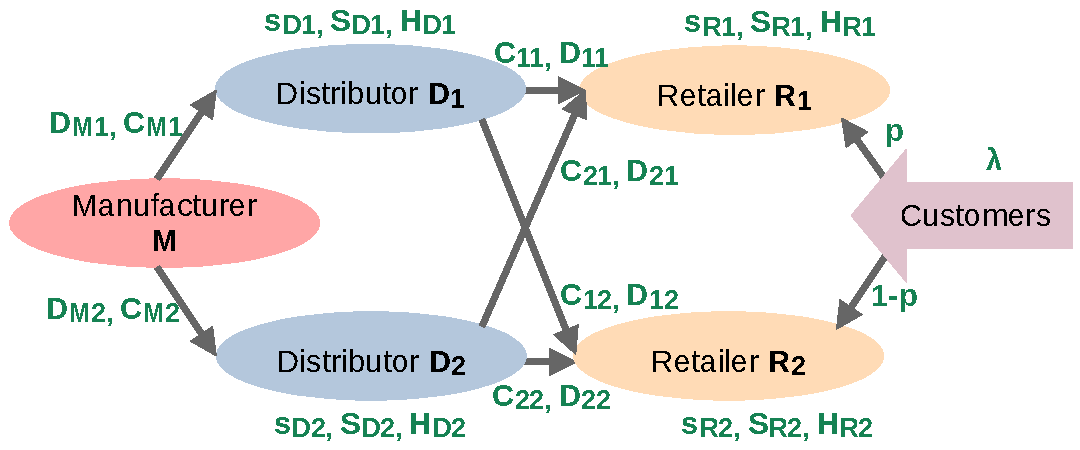
\includegraphics[width=0.47\textwidth]{image/SupplyChain.pdf}
   %{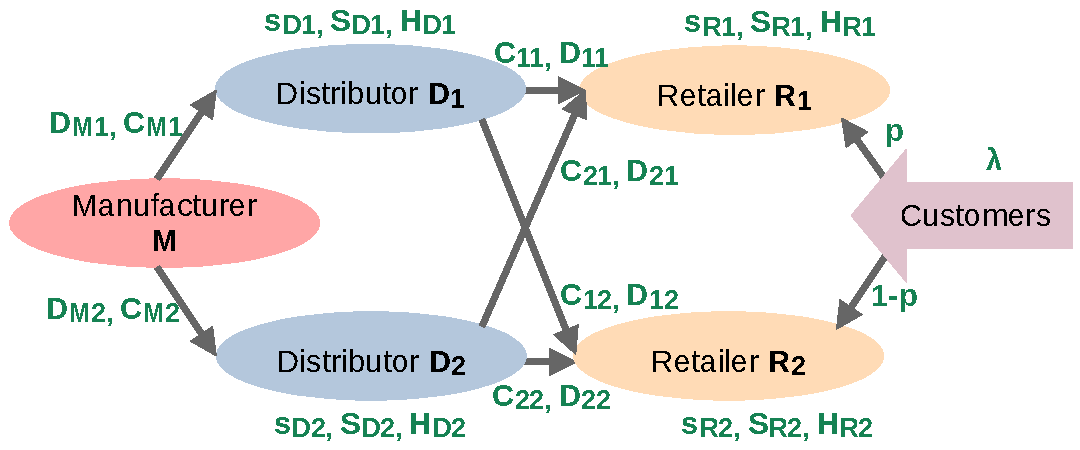
\epsfig{file = image/SupplyChain.pdf, width = \textwidth}}
     \caption{Supply chain network example. Parameters of each node are indicated in green.}
  \label{fig:simple_supply_chain_net}
  \end{figure}
%
 We assume that each item sold to the end customer generates a profit $P$. The transport delay, cost and holding cost values are assumed to be known/fixed based on data with reasonable values assumed for this case study. The inventory threshold and reorder parameters $s,S$ at each node are assumed to be the design variables for our optimization problem, with fixed bounds.
 %and their bounds are summarized in Table \ref{tab:param_val}. 
 The goal is to find optimal values of the inventory threshold and restock levels such that the net average profit of this system is maximized.  
 %
 %\begin{table}[h]\fontsize{9pt}{10pt}\selectfont
%\begin{table}[]
%\caption{The Supply chain design parameters, their bounds and values}\label{tab:param_val}
%\centering
%
%\begin{tabular}{|c|c|c|llll|}
%\hline
%\begin{tabular}[c]{@{}c@{}}Design\\ Parameters\end{tabular} & \begin{tabular}[c]{@{}c@{}}Lower\\ Bound\end{tabular} & \begin{tabular}[c]{@{}c@{}}Upper\\ Bound\end{tabular} & \multicolumn{4}{c|}{Values}                                                          \\ \hline
%$S_{R1}$                                                    & 350                                                   & 500                                                   & \multicolumn{1}{l|}{350} & \multicolumn{1}{l|}{400} & \multicolumn{1}{l|}{450} & 500 \\
%$s_{R1}$                                                    & 100                                                   & 250                                                   & \multicolumn{1}{l|}{100} & \multicolumn{1}{l|}{150} & \multicolumn{1}{l|}{200} & 250 \\
%$S_{R2}$                                                    & 350                                                   & 500                                                   & \multicolumn{1}{l|}{350} & \multicolumn{1}{l|}{400} & \multicolumn{1}{l|}{450} & 500 \\
%$s_{R2}$                                                    & 100                                                   & 250                                                   & \multicolumn{1}{l|}{100} & \multicolumn{1}{l|}{150} & \multicolumn{1}{l|}{200} & 250 \\
%$S_{D1}$                                                    & 600                                                   & 750                                                   & \multicolumn{1}{l|}{600} & \multicolumn{1}{l|}{650} & \multicolumn{1}{l|}{700} & 750 \\
%$s_{D1}$                                                    & 350                                                   & 500                                                   & \multicolumn{1}{l|}{350} & \multicolumn{1}{l|}{400} & \multicolumn{1}{l|}{450} & 500 \\
%$S_{D2}$                                                    & 600                                                   & 750                                                   & \multicolumn{1}{l|}{600} & \multicolumn{1}{l|}{650} & \multicolumn{1}{l|}{700} & 750 \\
%$s_{D2}$                                                    & 350                                                   & 500                                                   & \multicolumn{1}{l|}{350} & \multicolumn{1}{l|}{400} & \multicolumn{1}{l|}{450} & 500 \\ \hline
%\end{tabular}


\begin{tabular}{|c|c|c|}
\hline
\begin{tabular}[c]{@{}c@{}}\textbf{Design}\\ \textbf{Parameters}\end{tabular} & \begin{tabular}[c]{@{}c@{}}\textbf{Lower}\\ \textbf{Bound}\end{tabular} & \begin{tabular}[c]{@{}c@{}}\textbf{Upper}\\ \textbf{Bound}\end{tabular} \\ \hline
$S_{R1}$                                                    & 350                                                   & 500                                                   \\ \hline
$s_{R1}$                                                    & 100                                                   & 250                                                   \\ \hline
$S_{R2}$                                                    & 350                                                   & 500                                                   \\ \hline
$s_{R2}$                                                    & 100                                                   & 250                                                   \\ \hline
$S_{D1}$                                                    & 600                                                   & 750                                                   \\ \hline
$s_{D1}$                                                    & 350                                                   & 500                                                   \\ \hline
$S_{D2}$                                                    & 600                                                   & 750                                                   \\ \hline
$s_{D2}$                                                    & 350                                                   & 500                                                   \\ \hline
\end{tabular}

%\end{table}
%
% The following segment outlines the fixed parameter values used in our study:
%\begin{itemize}
%    \item The arrival rate of the customers ($\lambda$) is fixed at 20 customers per day.
%    \item The probability of a customer buying from retailer $R_1$ is  $p = 0.5 $ (So the probability of a customer buying from $R_2$ is $(1-p)=0.5$).
%    \item The inventory holding costs for retailers are $H_{R1} = H_{R2} = 10$ units, and for distributors, are $H_{D1} = H_{D2} = 1$ units.
%    \item The delivery costs from a distributor to a retailer are listed  as $C_{11} = 5000$, $C_{12} = 6000$, $C_{21} = 7000$, and $C_{22} = 5500$ units.
%    \item The delivery delays to deliver from distributor $i$ to retailer $j$ are $D_{11} = 2$ days, $D_{12} = 3$ days, $D_{21} = 3$ days, and $D_{22}=2$ days, respectively.
%    \item Finally, the delivery costs from manufacturer to distributors are $C_{M1} = C_{M2} = 500$, and delays are $D_{M1} = 7$ days, and $D_{M2} = 8$ days, respectively. 
%    \item $P = 100$ units is the profit generated per item the retailer sells.
%\end{itemize}
%     
%
%
%The parameter values for inventory thresholds and capacities are adjustable and not predetermined. Assuming variable values for the inventory thresholds and capacities is reasonable as the retailer or distributor controls them to ensure the product's availability. \tablename~ \ref{tab:param_val} summarises the ranges of values for supply chain parameters $(S,s)$.
%The range of values these parameters can take are as follows: \\ 
%$S_{R1} \in [350,500]$, $s_{R1} \in [100,250]$, $S_{R2} \in [350,500]$, $s_{R2} \in [100,250]$, $S_{D1} \in [600,750]$, $s_{D1} \in [350,500]$, $S_{D2} \in [600,750]$, and $s_{D2} \in [350,500]$.
%
The model has been implemented by writing a basic, configurable inventory-node class and a few other classes for modeling customer arrivals and monitoring.  The concurrent behavior of these nodes is described using a \textit{Process} construct in Python's SimPy library \cite{SimPy}.  The individual nodes, such as retailers and distributors, are implemented as derived classes that are instantiated into the system model by passing their respective parameter values and interconnected to model the supply chain's structure.  These classes form a part of InventOpt's current component library. The simulation length and the randomization seed can be specified, and each simulation run generates a detailed log (for validation and insight) and an output summary consisting of performance metrics such as the average (per-day) cost of running this supply chain (which can be attributed to the holding and transport costs), the average per-day income from the sale of items and the net average profit (denoted as $P_{net}$). 

\subsection{Design Space Exploration}

%\textbf{{Computational Cost and Estimation Accuracy:}}
For a given point in the design space, say $X=(x_1,x_2,\dots,x_7)$, $f(X)$ denotes the objective function to be minimized. In our case study, $f(X)$ is the negative of the average (per-day) net profit. A single simulation run of length $L$ days provides an estimate of $f(X)$. Since the model is stochastic in nature, individual simulation runs with distinct randomization seeds will yield slightly differing outcomes. An estimate for $f(X)$ can be obtained by averaging the results across multiple (say $N$) simulation runs with distinct randomization seeds. The accuracy of a performance estimate increases with $L$ and $N$. However, the computational cost grows directly as $L\times N$. This limits the number of design points that can be evaluated, given a fixed computational budget. To assess the trade-off between the measurement accuracy and computational cost, we consider a single point in the center of the design space and plot the Relative Standard Error (RSE) in the performance estimate obtained using $N$ simulation samples, each of length $L$.  The RSE is a measure of accuracy and reduces as the square root of $N$ (${RSE}\propto {1}/{\sqrt(N)}$) since the sample average is normally distributed. Further, the RSE reduces with $L$ since the objective function is defined to be a long run average measure for a model that has a steady-state behavior. Figure \ref{fig:compute_effort} presents a plot of the RSE values measured with respect to $L$ and $N$.  

\begin{figure}[!h]
  \vspace{-0.2cm}
  \centering
   %\includegraphics[scale=0.40]{image/supply_chain_nemon.png}
   {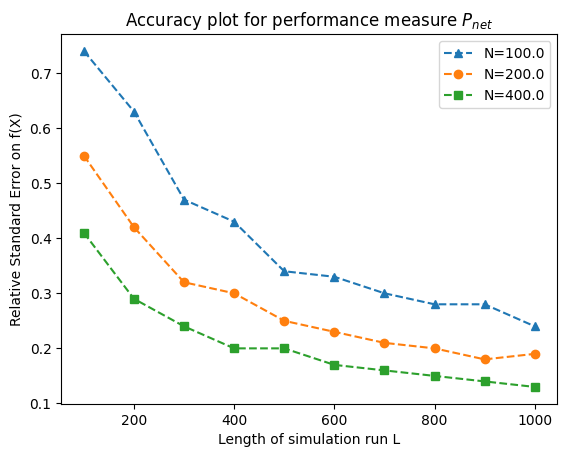
\epsfig{file = image/rse_vs_sim_len.png, width = 0.44\textwidth}}
  %\caption{This figure illustrates the trade-off between the computational effort and the accuracy of the expected performance measure $P_{net}$.}
  \caption{Relative Std Error (RSE) in simulation-based performance estimate as a function of simulation run length $L$ and the number of samples $N$}
  \label{fig:compute_effort}  
\end{figure}

 The plot allows us to understand the accuracy versus computational cost trade-off and budget the available computational time for design spacey exploration. We select the simulation length $L$ to be 720 days and the number of simulation samples $N$ to be 60, for a reasonable accuracy (RSE = 0.34\%). This corresponds to a serial (single-threaded) computational time of \textbf{130 seconds} on a modern x86 based workstation. Thus, estimating the objective function value $f(X)$ at any given point $X$ takes approximately \textbf{130 seconds} of computational time.
 
  To gain insights on how the objective value varies with each decision parameter, we perform design space exploration by taking simulation-based performance estimates at multiple points along a regular grid in the design space. Along each axis we consider 4 equi-spaced points. This results in a total of $4^8 = 65536$ design points at which we measure $f$.  Each measurement takes 130 seconds and thus the entire exploration requires approximately \textbf{96 days} of serial computational time. We perform  simulations in parallel on a 64-core x86-based rack-server using parallel execution scripts. With a speed-up of $64$x, the design exploration could be completed in approximately two days. 
 The measured data can provide valuable insights on how each design variable affects the performance. However the data is multi-dimensional. To visualize the simulation data, we have built a GUI tool that allows the user to upload measured data as a comma-separated-values (csv) file, and observe the function values as 3D slices, by selecting two axes at a time and varying the values of other axes via interactive sliders. This allows a user to visualize trends in the objective function. Aside from incorporating this functionality into InventOpt, we have also deployed this component as a standalone, cloud-hosted free tool called \textbf{DATAvis} (\texttt{https://datavis.streamlit.app}). Figure 
 %\ref{fig:DataVis_param_select} and 
 \ref{fig:DataVis_slice} shows a screenshot of the data visualization tool. 


%\begin{figure}[h]
 %   \begin{frame}{
 %   %\vspace{-0.2cm}
 %   \centering {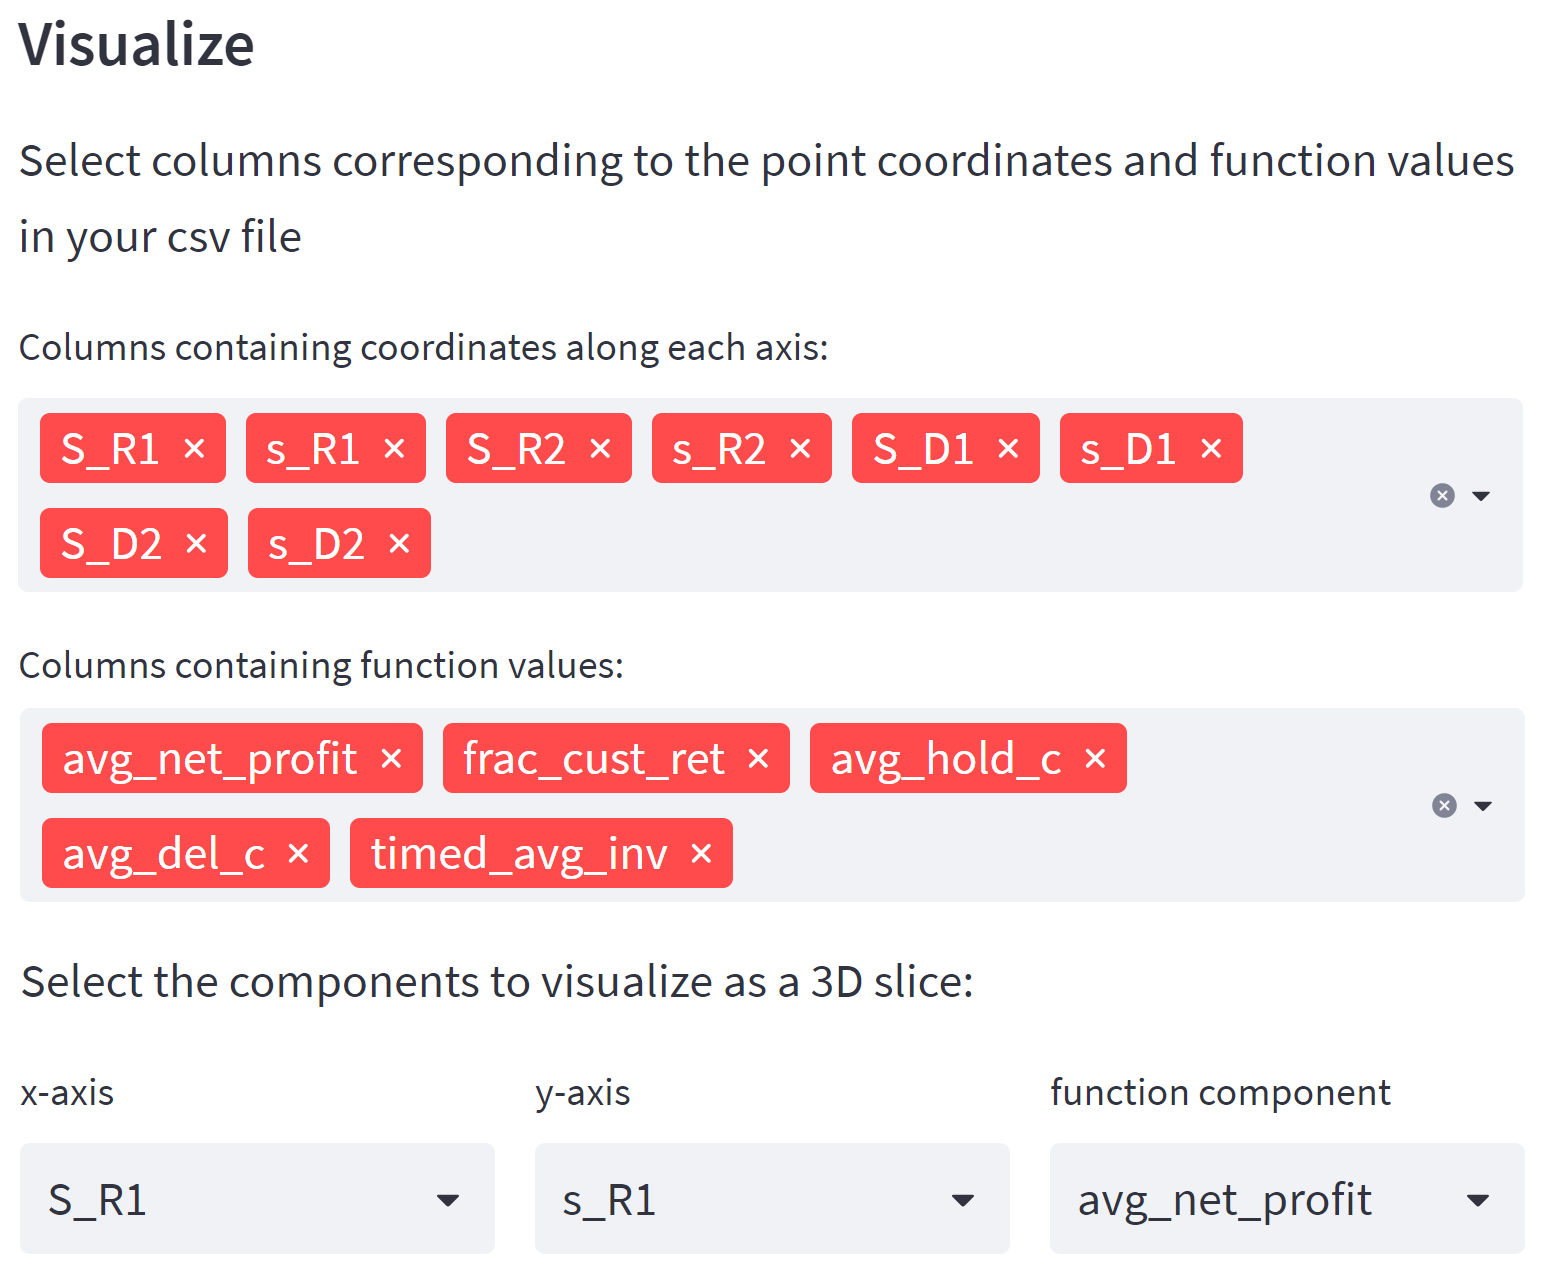
\epsfig{file = image/DataVis_params.png, width = 0.48\textwidth}}  
 %   }
 %   \end{frame}
 % \caption{Screenshot of \textit{DATAvis} showing selection of input and output axes from a csv data file for visualization}
 % \label{fig:DataVis_param_select}
  %\vspace{-0.1cm}
%\end{figure}

\begin{figure*}[!t]  
  \hspace*{1.5cm}
  \begin{frame}{
    %\vspace{-0.2cm}
    \centering {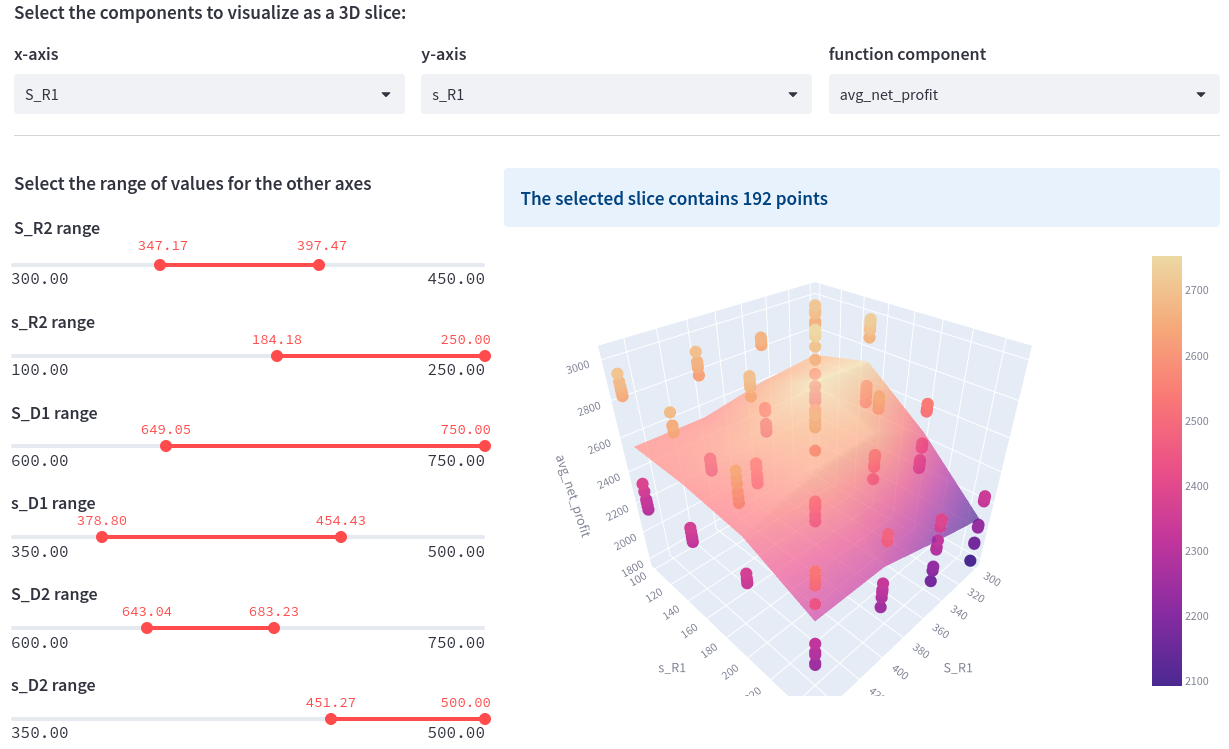
\epsfig{file = image/DataVis_slice.png, width = 0.85\textwidth}}
    }
  \end{frame}
  \caption{The \textit{DATAvis} tool allows a user to visualize multi-dimensional data as 3D slices by selecting two axes at a time and varying the values of other axes (at which the slice is taken) via interactive sliders. The GUI interface supports zooming/rotating the plot}
  \label{fig:DataVis_slice}
  %\vspace{-0.1cm}
\end{figure*}




\subsection{Meta-model Based Optimization} The next steps in our case study are to perform optimization and arrive at a general approach and design choices for InventOpt. These choices are with regards to the meta-model type, the number of data points needed for building a reasonably accurate meta-model and the choice of optimizer. To perform this exploration, we first find optimal points in the design space via a near-exhaustive evaluation approach. From the set of $4^8$ data points, we select good regions in the design space, and perform fine-grained sampling in its neighbourhood, comparing the objective values at each point to arrive at a point $X\rq$ which we consider as a reference solution. We use this as a means of evaluating the performance of the meta-model based approach with varying choices for the meta-model and optimizer pairs. A meta-model $g(X)$ provides an approximation to the original objective function $f(X)$, but allows significantly faster evaluation.
%
\begin{table*}[!h]\centering \fontsize{9pt}{10pt}\selectfont %\setlength{\tabcolsep}{2pt}
\caption{Results obtained using multiple optimizers over a GPR meta-model built using varying sizes of training data.}\label{tab:obtained_results}
% Please add the following required packages to your document preamble:
% \usepackage{multirow}
\begin{tabular}{|l|l|l|r|r|r|r|}
\hline
\multicolumn{1}{|c|}{\textbf{\begin{tabular}[c]{@{}c@{}}Training \\ Dataset\\ Size\end{tabular}}} & \multicolumn{1}{c|}{\textbf{MSE}} & \multicolumn{1}{c|}{\textbf{Optimizer}} & \multicolumn{1}{c|}{\textbf{\begin{tabular}[c]{@{}c@{}}Optimum\\ Objective\\ Value\end{tabular}}} & \multicolumn{1}{c|}{\textbf{\begin{tabular}[c]{@{}c@{}}Avg Number\\ of $g(X)$ \\ Evaluation\end{tabular}}} & \multicolumn{1}{c|}{\textbf{\begin{tabular}[c]{@{}c@{}}Avg Time to \\ Compute $g(X)$\\ (seconds)\end{tabular}}} & \multicolumn{1}{c|}{\textbf{\begin{tabular}[c]{@{}c@{}}Distance \\ to Reference\\ Solution $X’$\end{tabular}}} \\ \hline
\multirow{4}{*}{\begin{tabular}[c]{@{}l@{}}25\%\\ (16,385 training\\ points)\end{tabular}}        & \multirow{4}{*}{0.0008}           & COBYLA                                  & 4203.5                                                                                            & 355                                                                                                        & 0.0239                                                                                                          & 156.5                                                                                                          \\ \cline{3-7} 
                                                                                                  &                                   & Powell                                  & 4327.5                                                                                            & 346                                                                                                        & 0.0297                                                                                                          & 10.0                                                                                                           \\ \cline{3-7} 
                                                                                                  &                                   & SLSQP                                   & 4203.5                                                                                            & 172                                                                                                        & 0.0321                                                                                                          & 156.5                                                                                                          \\ \cline{3-7} 
                                                                                                  &                                   & Nelder-Mead                             & 4296.1                                                                                            & 861                                                                                                        & 0.0294                                                                                                          & 105.9                                                                                                          \\ \hline
\multirow{4}{*}{\begin{tabular}[c]{@{}l@{}}50\%\\ (32,768 training\\ points)\end{tabular}}        & \multirow{4}{*}{0.0015}           & COBYLA                                  & 4736.3                                                                                            & 318                                                                                                        & 0.0726                                                                                                          & 109.0                                                                                                          \\ \cline{3-7} 
                                                                                                  &                                   & Powell                                  & 4780.6                                                                                            & 348                                                                                                        & 0.0635                                                                                                          & 10.0                                                                                                           \\ \cline{3-7} 
                                                                                                  &                                   & SLSQP                                   & 4736.3                                                                                            & 149                                                                                                        & 0.0587                                                                                                          & 109.1                                                                                                          \\ \cline{3-7} 
                                                                                                  &                                   & Nelder-Mead                             & 4736.3                                                                                            & 878                                                                                                        & 0.0987                                                                                                          & 109.1                                                                                                          \\ \hline
\multirow{4}{*}{\begin{tabular}[c]{@{}l@{}}75\%\\ (49,152 training\\ points)\end{tabular}}        & \multirow{4}{*}{0.0037}           & COBYLA                                  & 4882.7                                                                                            & 339                                                                                                        & 0.0685                                                                                                          & 157.5                                                                                                          \\ \cline{3-7} 
                                                                                                  &                                   & Powell                                  & 5082.1                                                                                            & 314                                                                                                        & 0.0717                                                                                                          & 10.3                                                                                                           \\ \cline{3-7} 
                                                                                                  &                                   & SLSQP                                   & 4882.7                                                                                            & 145                                                                                                        & 0.0775                                                                                                          & 157.5                                                                                                          \\ \cline{3-7} 
                                                                                                  &                                   & Nelder-Mead                             & 5082.1                                                                                            & 869                                                                                                        & 0.0764                                                                                                          & 10.2                                                                                                           \\ \hline
\end{tabular}
\end{table*}

We build NN and GPR meta-models for this case study and compare the results generated using each of them. The meta-model parameters were tuned separately. 
%For the NN meta-model the number of hidden layers is fixed to 4, with 32 neurons in each layer. For the GPR model, we use an RBF kernel with length parameter 1 with bounds $(30,60)$. 
Out of the $4^8$ points, we select random subsets consisting of 25\%, 50\% and 75\% points as the training data, and the remaining points as test data to evaluate each meta-model. For each choice we report the extent of the match with the test points as a mean squared error (MSE), summarized in Table \ref{tab:obtained_results}. Python's \texttt{scikit-learn} library \cite{scikit-learn} was used for building the meta-models. 
%
The average computational time for building a GPR meta-model varied between 1000-7000 seconds depending on the training set size. For a NN model, the time for building and training the NN model varied from 300 to 1500 seconds. 
%
Once a meta-model is built, continuous, gradient-based optimizers can be applied over it to quickly identify promising regions in the design space. To arrive at a choice of optimizer for InventOpt, we consider multiple optimizers available in Python's SciPy library that are well-suited for this class of problems. The optimizers are listed in Table \ref{tab:obtained_results}. \textit{COBYLA} and \textit{Powell} are trust region-based optimization methods while \textit{SLSQP} and \textit{Nelder-Mead} are gradient-based methods and are popular choices for black-box optimization problems. We choose to use local optimizers rather than global optimizers because the idea is to utilize gradient information to quickly converge to regions of interest. One can use global optimizers such as Simulated Annealing which are more suited when the objective function is erratic or lacks trends. While this case study only considers local optimizers, we plan to incorporate a wider choice of optimizers in the InventOpt tool in future. Since the objective function may be non-convex we perform multiple optimization runs with random starting points for each optimizer.  Figure \ref{fig:convergence_plots} shows the convergence trends for each of these optimizers. Each subplot shows 20 optimization runs with distinct, randomly chosen starting points. The plot shows how the lowest $g(X)$ value found varies as the number of objective evaluations increases and presents a rough, visual estimate of the average convergence time for each optimizer. We observe that several runs in SLSQP and Powell converge faster,  though COBYLA and Nelder-Mead are resilient to noise. 
%
We observed that for the NN model the quality of results did not improve significantly with the size of training data, and the GPR model yielded considerably better results compared to the NN model. This may be because of the local minima inherently present in the NN model. The results for the GPR model are listed in Table \ref{tab:obtained_results} and summarized next.
%
%We identify the optimum reported by these results as a promising region and perform one more iteration. We narrowed the parameter ranges and restricted the search to a smaller region in the design space. Each parameter $S$ and $s$ are restricted to four equispaced values within these ranges. The maximum in this region is found at $X' = [S_{R1}=320, s_{R1}=130, S_{R2}=325, s_{R2}=125, S_{D1}=735, s_{D1}=480, S_{D2}=735, s_{D2}=475]$ with $f(X') = 3546.26$. 
The last column in Table \ref{tab:obtained_results} shows the Euclidean distance between the optimum found by an optimizer (choosing the best among the 20 independent runs) and $X'$ (the reference solution).  
%

%\end{landscape}
%The ranges for the parameters $S$ and $s$  are adjusted to $S_{R1} \in [310,325], s_{R1} \in [115,130], S_{R2} \in [310,325], s_{R2} \in [115,130], S_{D1} \in [720,735], s_{D1} \in [470,485], S_{D2} \in [720,735], s_{D2} \in [470,485]$.  We execute the simulation model with the input parameter values restricted to this region to identify the maximum within this constrained design space. It is observed to be present at $X' = [320, 130, 325, 125, 735, 480, 735, 475]$ with $f(X') = 3546.26$. The results were again visualised using the \textit{DataVis} tool. The meta-model-based optimization process was repeated for this new data set. However, the obtained results did not show any significant improvement in the optimum $X'$ found. The following section presents a comprehensive analysis of the results obtained from the case study and the insights derived from it.
%The present study employs the Bayesian Optimization method to estimate the optimal input parameter values that maximize the \textit{surplus} of the supply chain. Gaussian Process Regression (GPR) and Neural Network (NN) meta-models are utilized to obtain the posterior distribution via the application of the Bayes rule. Subsequently, various optimizers instead of acquisition functions are employed to determine the next promising region. A sampling of a limited number of points within the promising region is performed, followed by the application of the process of meta-model-based optimization. This iterative approach is repeated until the optimal solution within the design space is achieved. The process is detailed below.
%The optimizers are applied to both the GPR and NN meta-models, utilizing randomly sampled training datasets of 25\%, 50\%, and 75\% of the generated data. The results are summarized in \tablename~\ref{tab:obtained_results}. The highlighted cell indicates the optimized value determined by the optimizer, which is observed to be outside the predefined boundaries. Such found optimum is discarded. A performance discrepancy is observed between the Nelder-Mead optimizer and the NN meta-model. The column `optimum $g(X)$' refers to the optimum $P_{net}$ found by the optimizer on the respective meta-model. The next column lists the execution time taken for an optimizer to converge. The last column $d(X,X')$ lists the Euclidean distance between optimum $X$ found by the respective optimizer and the original optimum $X'$ mentioned below.
%The outcomes indicate that the maximum surplus values reported substantially deviate from the previously identified value of 3462.27, representing the maximum value in data obtained by running the simulation model. In addition, the reported optimal input parameter values exhibit considerable differences. These observations prompt redirecting the search for the optimum towards a more narrowly defined region, where a few additional points are sampled. This constitutes one iteration of the Bayesian optimization process.

\subsection{Results and Insights}
Observations from the meta-model based optimization case study show that the GPR model performs significantly better than the NN model in terms of the quality of solutions found. This could be attributed to the non-smooth approximation surface in the NN model. We observe that the quality of results obtained with the NN model do not show any significant improvement with respect to the training set size. However the NN model was found to be about 3x to 5x faster to train/build compared to the GPR model. A more exhaustive evaluation of NN models with other architectures needs to be performed in future. The GPR meta-model showed improved accuracy (indicated by the MSE with respect to the test data) with increasing training data-set sizes. The results for the GPR model are summarized in Table \ref{tab:obtained_results}. The GPR models provide a smoother surface for optimization and gradient-based optimizers such as Powell and COBYLA are found to perform well over it. 
%
\begin{figure}[!h]
  \vspace{-0.2cm}
  \centering
   %\includegraphics[scale=0.40]{image/supply_chain_nemon.png}
   {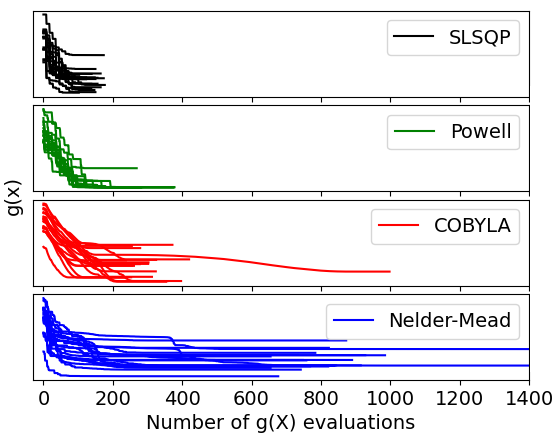
\epsfig{file = image/75gpr-convergence-graphs.png, width=0.42\textwidth}}
  %\caption{This figure illustrates the trade-off between the computational effort and the accuracy of the expected performance measure $P_{net}$.}
  \caption{Convergence plots for optimizers applied on the GPR meta-model.   The range of objective values $g(X)$ on the y-axis for all of the plots is from -5000 to -3000.}
  \label{fig:convergence_plots}
\end{figure}

The number of data points required for building the meta-model grows exponentially with the number of decision variables. Also, the computational time for fitting the meta-model grows with increasing training set size. We observe that the promising regions found by the GPR meta-models built with different training sizes align well, indicating that an incremental sampling approach to design space exploration can be used. A GPR meta-model can be initially built using a small number of training samples, optimizers could be applied over it to locate promising regions, and these regions could be explored further using fine-grained sampling, repeated in an iterative manner. 
%
Across the set of optimizers explored in this case study, we observed that the implementation of Nelder Mead in SciPy library does not accept parameter bounds as arguments since it is primarily intended for unconstrained optimization. This leads to several runs producing solutions that are outside acceptable bounds. Although there are ways to overcome this by modifying the objective function to introduce penalties for out-of-bound solutions, we observe that COBYLA, Powell and SLSQP methods can accept bounds and find good solutions.  These methods also show good convergence results. We observe that several runs of Powell and SLSQP converge to good solutions rapidly. 

In summary, this case study provides useful insights for design choices in the implementation of InventOpt and justifies the use of an iterative meta-model based approach for a similar class of problems in supply chain design and optimization. We plan to generalize and incorporate the steps performed in this case study into configurable, user-guided semi-automated routines in the InventOpt tool-set.
 
%Increasing the training data's size did not improve the obtained optimum for the NN meta-model. It performed poorly with the Nelder-Mead optimizer and yielded out-of-bound results. However, the average time to build a NN meta-model is much less than GPR. The NN meta-model with 50\% training data and Powell, SLSQP optimizers showed promising results and redirected the search to a promising region.

%The optimal value obtained by the GPR meta-model trained on 25\% of the generated data is consistent with that obtained by the GPR meta-model trained on 75\%. The optimum value $g(X)$ reported by GPR is $P_{net} \approx 5082$, which is higher than the actual optimum found in this region, which is approximately equal to $3546$.  In the case of the NN meta-model, the model with 50\% training samples shows good results where COBYLA, SLSQP and Powell converge to a point near the actual optimum. However, the Nelder-Mead optimization method does not require bounds, resulting in frequently obtaining solutions outside the acceptable range. This optimizer exhibited poor performance when applied to NN meta-models, yielding out-of-bounds results, which were discarded. The case study results indicate that the GPR meta-model outperforms NN for the given problem. However, it is worth noting that the computational cost of constructing the GPR meta-model is higher than NN. While GPR successfully directs the search for the optimum to the promising region, the reported optimum value differs from the actual one.

%We have considered a vast design space of $150^8$ design points for the case study, where each simulation takes 130 seconds. The computational cost can be huge when applying optimizers directly to the simulation model. However, deciding the number of sampling points, the meta-model, and its parameter values are critical for meta-model-based optimization. The case study demonstrates a systematic decision-making process facilitated by a visual interface. The insights in the case study can be used and applied to tackle similar problems. 

 %The GPR model is recommended when tackling inventory optimization problems in a supply chain as it performed better than the NN meta-model for the case study. The results show that utilizing 25\% of the data samples is sufficient for the GPR meta-model for leveraging the gradient information. The number of points to sample for building the meta-model is correlated to the design space's size. And GPR meta-model works well with the small subset of design space points as training points provided that the meta-model parameters are tuned to obtain a good fit over the original data points. The meta-model parameters can be adjusted iteratively by visualizing the fit in the \textit{DataVis} tool and accepting a fit with a reasonably small MSE. Powell and SLSQP local optimizers show improved performance with GPR meta-model due to their effective utilization of the gradient information exploited by the meta-model.



%The experiments showed that the GPR meta-model performs better than the NN meta-model. GPR shows the improved distance from the reference solution with increased training data size. It is likely due to the NN meta-model not always producing a smooth surface. However, GPR produces a smooth approximation surface to the training data, which aids in exploiting the gradient information for the optimizers.

%When considering sample size selection, the NN meta-model displayed relatively better outcomes when trained on 50\% of the samples. Conversely, the GPR meta-model showed improved performance as the training data size increased. Notably, the promising region reported by the GPR meta-model with 25\% training data aligns with the 75\% data. This indicates that a 25\% sample size is adequate for the GPR meta-model to identify suitable promising regions in our case.



%The smoothness of the approximation surface generated by GPR can be inferred from the similarity of the optimums reported by the GPR with 25\%, 50\% and 75\% training samples. It indicates that utilizing 25\% of the data samples is sufficient for the GPR meta-model for leveraging the gradient information and effectively directing the search for the optimal solution towards the promising region.
%In order to improve the accuracy of the meta-model, a larger number of points can be sampled to obtain a better fit. However, this approach would increase the time complexity of the overall optimization process. In the case study, random and regular grid sampling was utilized. However, other sampling techniques can be explored and experimented with to determine a better number of sample points. Choosing a meta-model for a given problem is a critical decision in the optimization process, and estimating the meta-model parameters is essential to obtain a good fit. 
%The optimization algorithms Powell and Nelder-Mead exhibited good performance with the GPR meta-model, while COBYLA performed well with the NN meta-model. It is necessary to conduct experiments with various optimizers when utilizing a particular meta-model, ultimately selecting the most effective one.




%%%%%%%%%% %%%%%%%%%% %%%%%%%%%% %%%%%%%%%% %%%%%%%%%% %%%%%%%%%% %%%%%%%%%% %%%%%%%%%% %%%%%%%%%% %%%%%%%%%% %%%%%%%%%% %%%%%%%%%% %%%%%%%%%% %%%%%%%%%%
\section{\uppercase{Results and Insights}}
\label{sec:results}
\paragraph{Results and Observations:} 
%observations
The optimal value obtained by the GPR meta-model trained on 25\% of the generated data is consistent with that obtained by the GPR meta-model trained on 75\%. The optimum value $g(X)$ reported by GPR is $P_{net} \approx 5082$, which is higher than the actual optimum found in this region, which is approximately equal to $3546$.  In the case of the NN meta-model, the model with 50\% training samples shows good results where COBYLA, SLSQP and Powell converge to a point near the actual optimum. However, the Nelder-Mead optimizer did not perform well with the NN meta-model. The case study results indicate that the GPR meta-model outperforms NN for the given problem. However, it is worth noting that the computational cost of constructing the GPR meta-model is higher than NN. While GPR successfully directs the search for the optimum to the promising region, the reported optimum value differs from the actual one.

We have considered a vast design space of $150^8$ design points for the case study, where each simulation takes 130 sec. The computational cost can be huge when applying optimizers directly to the simulation model. However, deciding the number of sampling points, the meta-model, and its parameter values are critical for meta-model-based optimization. The case study demonstrates a systematic decision-making process facilitated by a visual interface. The insights in the case study can be used and applied to tackle similar problems. 

\paragraph{Insights:} The GPR model is recommended when tackling inventory optimization problems in a supply chain as it performed better than the NN meta-model for the case study. The results show that utilizing 25\% of the data samples is sufficient for the GPR meta-model for leveraging the gradient information. The number of points to sample for building the meta-model is correlated to the design space's size. And GPR meta-model works well with the small subset of design space points as training points provided that the meta-model parameters are tuned to obtain a good fit over the original data points. The meta-model parameters can be adjusted iteratively by visualizing the fit in the \textit{DataVis} tool and accepting a fit with a reasonably small MSE. Powell and SLSQP local optimizers show improved performance with GPR meta-model due to their effective utilization of the gradient information exploited by the meta-model.

%The smoothness of the approximation surface generated by GPR can be inferred from the similarity of the optimums reported by the GPR with 25\%, 50\% and 75\% training samples. It indicates that utilizing 25\% of the data samples is sufficient for the GPR meta-model for leveraging the gradient information and effectively directing the search for the optimal solution towards the promising region.
%In order to improve the accuracy of the meta-model, a larger number of points can be sampled to obtain a better fit. However, this approach would increase the time complexity of the overall optimization process. In the case study, random and regular grid sampling was utilized. However, other sampling techniques can be explored and experimented with to determine a better number of sample points. Choosing a meta-model for a given problem is a critical decision in the optimization process, and estimating the meta-model parameters is essential to obtain a good fit. 
%The optimization algorithms Powell and Nelder-Mead exhibited good performance with the GPR meta-model, while COBYLA performed well with the NN meta-model. It is necessary to conduct experiments with various optimizers when utilizing a particular meta-model, ultimately selecting the most effective one.

%This reasonably complex case study shows that multi-dimensional design space, meta-models and optimizers exploration and visualization can be done iteratively and step-by-step to find the optimal.  Validation plays a vital role in each step of this process. It is essential to have a tool that automates and assists the user with visual aids in making critical decisions. 

\paragraph{Conclusion:} We presented a detailed case study that allowed us to arrive at an approach for meta-model-based optimization for supply chains. The case study illustrated modeling of a supply chain network, estimation of the time complexity of the experiment and number of samples to build meta-models, and the choice of meta-models and optimizers to find optimum and promising regions reasonably quickly. We plan to implement this entire approach into the InventOpt tool-set. We have already built a component of the tool-set to visualize multidimensional data called \textit{DataVis}. This study serves as guidelines for design and implementation of InventOpt tool.

\bibliographystyle{apalike} 
{\small \bibliography{example}}

\end{document}
